\documentclass{article}

\usepackage{lipsum}
\usepackage{color}
\usepackage{amsmath}
\usepackage{graphicx}
\usepackage[utf8]{inputenc}

\setlength{\arrayrulewidth}{1mm}
\setlength{\tabcolsep}{18pt}
\renewcommand{\arraystretch}{1.5}


\title{Microcontrollers \& Embeded System Design ~\textbf{\\CSE 315}}
\author{Md Awsaf Alam}
\date{\today}

\begin{document}

\maketitle
% \lipsum[1-3]
\newpage

\tableofcontents

\newpage


\section{8086/8088 Hardware Specifications}

\subsection{Introduction}
\label{sec:intro_text}
% This is the \textbf{first} CSE 300 class in Jan 2018 term.
% This is a new \textcolor{red}{\textbf{line}}.

\begin{description}
    \item[$\overline{RD}$]
    \begin{itemize}
        \item  Whenever this pin goes to logic 0, the data bus becomes receptive to data from the memory or I?O devices
            connected to the system.
        \item Floats to high impedence state during a hold acknowledge
    \end{itemize}

    \item[READY]
    \begin{itemize}
        \item $\mu p$ enters into \textbf{WAIT} state and remains idle if this pin is at logic 0
        \item No effect on operations of $\mu p$, if this pin is at logic 1
    \end{itemize}


    \item[INTR]
    \begin{itemize}
        \item  Used to request a h/w interrupt
        \item  If INTR is held high when $IF = 1$, the $\mu p$ enters an interrupt acknowledge cycle
        ( $\overline{INTA}$ becomes active) after completion of the current instruction
    \end{itemize}

    \item[$\overline{TEST}$]
    \begin{itemize}
        \item  An input that is tested by the WAIT instruction
        \item  If TEST is logic 0, the WAIT instruction functions as NOP
        \item If TEST is logic 1, the WAIT instruction waits for \textbf{TEST} to become 0
    \end{itemize}

   \item[NMI]
   \begin{itemize}
       \item Non markable interrupt pin
       \item Similar to the \textbf{INTR} except that NMI does not check IF (whether it is 1)

   \end{itemize}

   \item[RESET]
   \begin{itemize}
       \item Causes the $\mu p$ to reset itself if this pin remains high for a minimum of four clocking periods
      \item whenever the up gets reset , it begins executing instructions at memory location \textbf{FFFFOH}
      and disables future interrupts by clearing IF
   \end{itemize}

   \item[CLK]
   \begin{itemize}
       \item  Provides the base timing signal to the up
       \item Clock signal must have at least 33\% duty cycle (high for the one-third
       of the clocking period and low for two-third of the period)

  \end{itemize}

  \item[VCC]
  \begin{itemize}
      \item Power supply input
      \item Provides $+5.0$ volt with 10\% tolerance to the up

  \end{itemize}

  \item[GND]
  \begin{itemize}
      \item 2 pins, both must be connected to ground

  \end{itemize}

  \item[MN/$\overline{MX}$]
  \begin{itemize}
      \item Selects either minimum mode or maximum mode operation of the up
  \end{itemize}


  \item[$\overline{BHE}$/S7]
  \begin{itemize}
      \item Bus high Enable
      \item Used in 8086 to enable the most signifant data bus bits (D15 - D8) during a read or
      write operations
      \item The state of S7 is always a logic 1
  \end{itemize}

\subsection{Minimum Mode Pins}

  \item[IO/$\overline{M}$ or M/$\overline{IO}$]
  \begin{itemize}
      \item Selects memory or I/O
      \item Indicates the $\mu p's$ address bus contains either a memory address or an I/O
      port address
      \item High impedence state during a hold acknowledge
  \end{itemize}

  \item[$\overline{WR}$]
  \begin{itemize}
      \item Indicates that the $\mu p$ is outputting data to a mem or I/O device
      \item Data bus contains valid data for memory or I/O during the time $\overline{WR}$ remains 0
  \end{itemize}

  \item[$\overline{INTA}$]
  \begin{itemize}
      \item  A response to the INTR input pin
      \item  Used to gate the interrupt vector number onto the databus in response to an interrupt request.
  \end{itemize}

  \item[$\overline{ALE}$]
  \begin{itemize}
      \item  Address Latch Enable
      \item Indicates that the $\mu p's$ address/ data bus contains address information
      \item The address can be a mem address or I/O port number
      \item ~[~Does \textbf{\underline{NOT}} float during a hold acknowledge~]
  \end{itemize}

  \item[DT/$\overline{R}$]
  \begin{itemize}
      \item  Data Transmit or Receive
      \item Indicates that the $\mu p's$ data bus is transmitting $( DT/\overline{R} = 1 )$ or
      receiving $( DT/\overline{R} = 0 )$ data.
      \item Used to enable external data bus buffers.
  \end{itemize}

  \item[DEN]
  \begin{itemize}
      \item Data bus enable
      \item Activates external data bus buffers.
  \end{itemize}

  \item[HOLD]
  \begin{itemize}
      \item Requests a direct memory access (DMA)
      \item If it is a logic 1, $\mu p$ stops executing S/W and places its address, data and control
      bus at high impedence state
      \item If it is a logic 0, the $\mu p$ executes S/W normally
  \end{itemize}

  \item[HLDA]
  \begin{itemize}
      \item Hold acknowledge
      \item Indicates that the $\mu p$ has entered the hold state
  \end{itemize}

  \item[$\overline{SSO}$]
  \begin{itemize}
      \item Equivalent to SO pin in maximum mode option of the $\mu p$
      \item It is combined with IO/$\overline{M}$ and DT/$\overline{R}$ to decode function of the current bus cycle
  \end{itemize}

\end{description}
\newpage
\subsection{Tables}

\begin{table}[h!]
\centering
\begin{tabular}{ |p{1cm}|p{1cm}|p{1cm}|p{3cm}|  }
\hline
IO/$ \overline{M} $ & DT/$ \overline{R} $ & $ \overline{SSO} $& Function   \\
\hline
0 & 0 & 0 & Interrupt acknowledge \\
0 & 0 & 1 & Memory read \\
0 & 1 & 0 & Memory write \\
0 & 1 & 1 & Halt \\
1 & 0 & 0 & Opcode fetch \\
1 & 0 & 1 & I/O read \\
1 & 1 & 0 & I/O write \\
1 & 1 & 1 & Passive inactive \\
\hline
\end{tabular}

\caption{Bus cycle status (8088) [Minimum mode]}
\label{table:1}
\end{table}

\begin{table}[h!]
\centering
\begin{tabular}{ |p{1cm}|p{1cm}|p{1cm}|p{3cm}|  }
\hline
$ \overline{S_2} $ & $ \overline{S_1} $ & $ \overline{S_0} $ & Function   \\
\hline
0 & 0 & 0 & Interrupt acknowledge \\
0 & 0 & 1 & I/O read \\
0 & 1 & 0 & I/O write \\
0 & 1 & 1 & Halt \\
1 & 0 & 0 & Opcode fetch \\
1 & 0 & 1 & Memory read \\
1 & 1 & 0 & Memory write \\
1 & 1 & 1 & Passive inactive \\
\hline
\end{tabular}

\caption{Bus control functions generated by the bus controller 8288 [~Maximum mode~]}
\label{table:2}
\end{table}

\section{Lecture - 3 }

\subsection{Maximum Mode Pins}
For using external coprocessors:
\begin{description}

    \item[$\overline{S2} , \overline{S1} and \overline{S0} $]
    \begin{itemize}
        \item Indicate the function of current bus-cycle
        \item Normally decoded by 8288 bus controllers
    \end{itemize}

    \item[$\overline{R1} / \overline{G1} and \overline{R0} / \overline{GT0} $]
    \begin{itemize}
        \item Request/grant pins
        \item Request Direct Memory Access
        \item Bi-Directional lines
        \item used to both request and grant a DMA operations
    \end{itemize}

    \item[$\overline{LOCK} $]
    \begin{itemize}
        \item Used to lock peripherals off the system
    \end{itemize}

    \item[$\overline{QS_1}  and \overline{QS0} $]
    \begin{itemize}
        \item Queue status bits
        \item Show status of the internal instructions queue
        \item Accessed by numeric coprocessor (8087)
    \end{itemize}

\end{description}

\begin{table}[h!]
\centering
\begin{tabular}{ |p{1cm}|p{1cm}|p{3cm}|  }
\hline
$ \overline{QS_1} $ & $ \overline{QS_0} $  & Function   \\
\hline
0 & 0 & Queue is idle \\
0 & 1 & First byte of opcode \\
1 & 0 & Queue is empty\\
1 & 1 & Subsequent byte of opcode \\
\hline
\end{tabular}

\caption{}
\label{table:4}
\end{table}

\subsection{Clock Generator (8284A)}
\begin{description}
  \item[Basic functions]
  \begin{itemize}
    \item Clock generation
    \item \textbf{RESET} synchronization
    \item READY synchronization
    \item TTL-level peripheral clock signal
  \end{itemize}
\end{description}
\newpage
\subsubsection{Pin diagram}
\begin{figure}[h!]
    \centering
    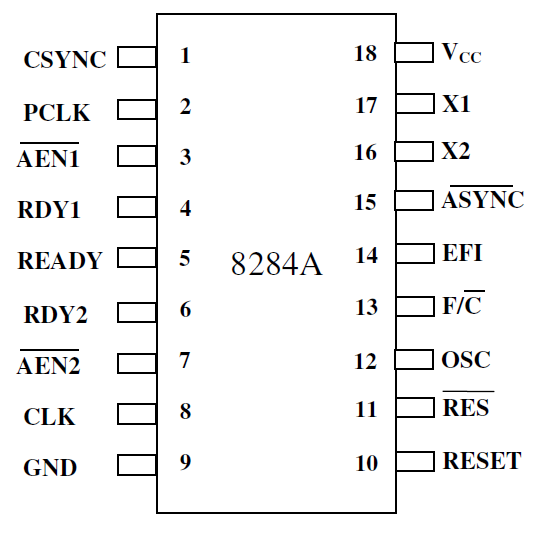
\includegraphics[width = 0.8\textwidth]{figures/8284A.png}
    \caption{Pin Diagram for Intel 8284A}
    \label{fig:bl}
\end{figure}

\subsubsection{Pin Functions}
\begin{description}

  \item[AEN1 and AEN2]
  \begin{itemize}
    \item Qualify the bus ready signals, RDY1 and RDY2 respectively
    \item wait states are generated by the \textbf{READY} pin of $\mu P$, which is controlled
    by $\overline{AEN1}$ and $\overline{AEN2}$ pins
  \end{itemize}

  \item[RDY1 and RDY2]
  \begin{itemize}
    \item Bus ready inputs
    \item Cause wait states in conjunction with $\overline{AEN1}$ and $\overline{AEN2}$ pins
  \end{itemize}

  \item[$\overline{ASYNC}$]
  \begin{itemize}
    \item Ready synchronization
    \item Selects either one or two stages of synchronization for RDY1 and RDY2 inputs

  \end{itemize}

  \item[READY]
  \begin{itemize}
    \item An output pin that connects to the $\mu P's$ READY input
    \item Synchronized with RDY1 and RDY2 inputs
  \end{itemize}

\end{description}


\end{document}
